\section{Искусственные нейронные сети}

\indent
\indent
Данная часть работы предназначена для читателя, не знакомого с 
искусственными нейронными сетями и способами их обучения. 
Здесь будут приведены теоретические 
основы глубокого обучения и рассмотрены сверточные архитектуры, 
используемые в дальнейшей работе.


\subsection{Перцептрон}

\indent
\indent
Начнем с рассмотрения одиночного нейрона
 --- перцептрона Розенблатта --- базового элемента, содержащегося в большинстве современных нейросетевых архитектур.
Перцептрон имеет несколько входов и один выход, значение на котором
вычисляется как взвешенная сумма значений входов 
(рисунок \ref{tikzpicture: perceptron}).
Кроме того, обычно
к выходному значению применяется сдвиг и некоторая нелинейная функция, 
называющаяся функцией активации нейрона. Ее предназначение мы обсудим позже.

\begin{figure}[h!]
    \begin{center}
   	    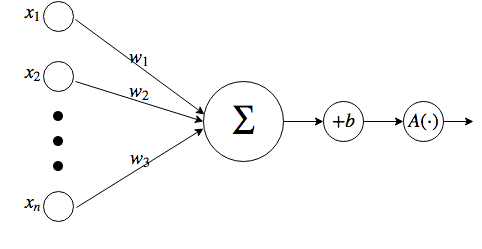
\includegraphics[width=0.6\linewidth]{Perceptron}
   	\end{center}
   	\caption{Схема работы одного отдельного нейрона.}
   	\label{tikzpicture: perceptron}
\end{figure}


\indent
\indent
Таким образом, значение на выходе нейрона задается
 выражением \ref{eq:perceptron}.

\begin{equation}\label{eq:perceptron}
    f(\vec{x}) = A(\sum_{i=1}^n x_i w_i + b)
\end{equation}


где $f(\vec{x})$ -- выходное значение нейрона, посчитанное для входов $x_i$,
$w_i$ -- весовые коэффициенты для каждого входа, $b$ -- параметр смещения, 
а $A$ --- нелинейная функция активации. Далее для упрощения повествования
положим $b \equiv 0$.

\subsection{Функции активации}

\indent
\indent
Существует множество различных функций активации, например, гиперболический
тангенс, логистическая сигмоида или \textit{ReLU}
соответственно, рисунок \ref{tikzpicture: activations}.

\begin{equation}\label{eq:activations}
	\begin{gathered}
	    A_{1}(x) = th(x) = \frac{e^x - e^{-x}}{e^x + e^{-x}},    \;   th’(x) = {1 - th(x)^2}  \\    
	    A_{2}(x) = \sigma(x) = \frac{1}{1 + e^{-2x}},   \;   \sigma’(x) = \sigma(x)(1 - \sigma(x)) \\
	    A_{3}(x) = ReLU = max(0, x),   \;   ReLU’(x) = \theta(x)
	\end{gathered}
\end{equation}
где $\theta(x)$ -- функция Хэвисайда.

\indent
\indent
Эти функции используются
для добавления нелинейных зависимостей между слоями многослойной модели.
Названные выше функции особенно популярны, 
так как значения их производных либо достаточно просты, либо легко 
выражаются через значения самих функций (выражение \ref{eq:activations}), 
что позволяет быстро вычислять значение производной.

\begin{figure}[h!]
	\begin{center}
		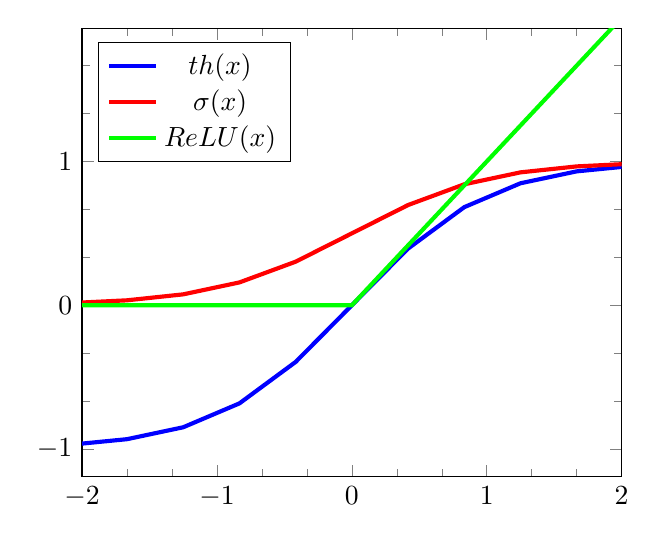
\begin{tikzpicture}
			\begin{axis} [
			    legend pos = north west, 
			    xmin = -2,
			    xmax = 2,
			    minor tick num = 2
			]
			\legend{ 
				$th(x)$, 
				$\sigma(x)$, 
				$ReLU(x)$
			};
			\addplot[blue, line width = 1.5] {tanh(x)};
			\addplot[red, line width = 1.5] {1 / (1 + e^(-2*x))};
			\addplot[green, line width = 1.5] {max(0, x)};
			\end{axis}
		\end{tikzpicture}
	\end{center}
\caption{Функции активации}
\label{tikzpicture: activations}
\end{figure}

\subsection{Полносвязная сеть}

\indent
\indent
Одиночный нейрон не способен выразить сложные зависимости в наборе
признаков $\vec{x}$, поэтому нейроны объединяют в слои, а их, в свою 
очередь, в многослойные сети. Рассмотрим сеть,
состоящую из двух слоев нейронов. Пусть количество входных признаков
равно $N$, количество нейронов скрытого слоя P,
а размер выхода -- M, рисунок \ref{tikzpicture: fc_net}. Такая архитектура, 
состоящая из простых линейных слоев, называется полносвязной.

\begin{figure}[h!]
    \begin{center}
   	    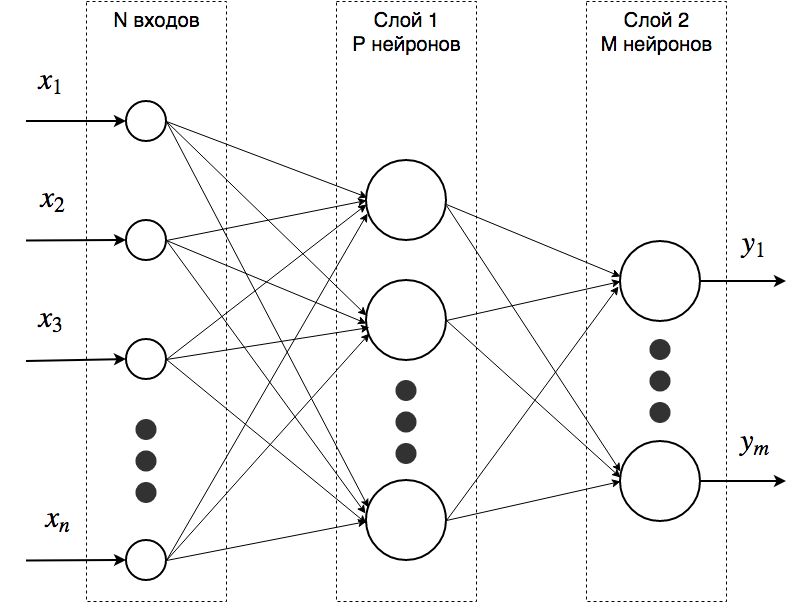
\includegraphics[width=0.9\linewidth]{FC_net}
   	\end{center}
   	\caption{Схема полносвязной нейронной сети.}
   	\label{tikzpicture: fc_net}
\end{figure}

Рассмотрев выражение \ref{eq:perceptron} можно увидеть, что 
совокупность значений нейронов на 1 слое может быть получена 
обычным матричным умножением матрицы весов
 $W^1$ размера $P \times N$ на значения входов $\vec{x}$.
После чего необходимо поэлементно применить 
функцию активации к получившимся значениям. Аналогично, значения нейронов
2 слоя получаются умножением весовой матрицы
$W^2$ размером $M \times P$ на выходы предыдущего слоя .
Таким образом, применение всей нейросети
ко входу $\vec{x}$ можно задать выражением \ref{eq:forward}.

\begin{equation}\label{eq:forward}
	   \vec{y} = A(W^{2} A(W^{1} \vec{x}))
\end{equation}
где $A(\cdot)$ -- применение нелинейности к каждому элементу входного 
вектора.

\indent
\indent
Если бы мы не добавляли после слоев нелинейность, то выражение \ref{eq:forward}
выродилось бы в простое умножение слева входного вектора $\vec{x}$ на матрицу
$W^{12} \equiv W^{2} W^{1}$. В этом случае модель не смогла бы выучить 
сложные нелинейные зависимости в данных, а добавление дополнительных слоев
не имело бы смысла, т.к. все они могут быть сведены к одной матрицей весов.

\indent
\indent
Отметим, что количество весов сети, состоящей из полносвязных слоев, растёт
мультипликативно от их размеров. Поэтому из-за больших вычислительных затрат
 на практике обычно не встречаются по-настоящему глубокие полносвязные архитектуры.
 Один из способов выразить сложные зависимости меньшим количеством слоев ---
 использование сверточных слоёв, о которых будет рассказано позднее.


\subsection{Функции потерь}
\label{section: losses}

\indent
\indent
Близость предсказания сети к правильным ответам оценивается
с помощью функции ошибки, так же называемой 
 функцией потерь \textit{(loss function)}. 
Например, для задачи регрессии в качестве функции потерь
может применяться сумма квадратов отклонений
 (выражение \ref{eq: se}),
 или, в более простом случае -- сумма разностей между выходами модели
  и правильными ответами (выражение \ref{eq:diff});
для задачи классификации обычно используют перекрестную энтропию 
(\textit{cross entropy}, выражение \ref{eq: cross_entropy}).


\begin{equation}\label{eq:diff}
    L_{diff}(\vec{y_{gt}}, \vec{y}) = \sum_{i=1}^M | y^{gt}_{i} - y_{i} |
\end{equation}

\begin{equation}\label{eq: se}
    L_{mse}(\vec{y_{gt}}, \vec{y}) = \frac{1}{2} \sum_{i=1}^M (y^{gt}_{i} - y_{i})^2
\end{equation}
где $\vec{y}$ -- предсказанный моделью $M$-мерный целевой вектор 
признаков, $\vec{y_{gt}}$ -- правильные значения признаков; в общем
случае в задаче регрессии признаки являются вещественными числами
 $\in (- \inf; + \inf )$.

\begin{equation}\label{eq: cross_entropy}
    L_{ce}(y_{gt}, \vec{y}) = - \sum_{i=1}^M \delta_{y_{gt}, i} \log{y_{i}}
\end{equation}
где $i$ -- метка класса (классы пронумерованы натуральными 
числами от $1$ до $M$),
$y_{gt}$ --  правильная метка класса
для рассматриваемого экземпляра данных;
$y_i$ -- предсказанная вероятность того, что 
экземпляру соответствует $i$-й класс;
$\delta_i$ -- символ Кронекера. 


\indent
\indent
Исходя из специфики решаемой задачи, можно составить и другие функции ошибок, но
они обязательно должны быть дифференцируемыми.
Это необходимо условие, чтобы использовать метод обратного распространения
ошибки для обучения модели.


\subsection{Обучение нейронных сетей}
% https://habr.com/ru/company/ods/blog/344116/
% https://ru.wikipedia.org/wiki/Метод_обратного_распространения_ошибки

\indent
\indent
Обучение нейронной сети -- это процесс изменения весовых
коэффициентов между нейронами, направленный на уменьшение
значения функции потерь на тренировочном наборе данных $\{ \vec{x} | \vec{y} \}$. 
Мы рассмотрим базовую реализацию такого процесса -- алгоритм 
стохастического градиентного спуска. Мы будем подавать на вход модели
размеченные тренировочные данные, объединенные в  небольшие партии 
-- батчи \footnote{\textit{Батчом} называется набор примеров, который передаётся
модели на обработку за один раз. При работе с изображениями размер батча 
обычно ограничивается размером памяти видеокарты,
на которой происходят вычисления.
Как правило, очередной шаг оптимизационной процедуры совершается после
прохождения батча, а не отдельного примера.}
Идея состоит в том, чтобы после каждой такой партии примеров
добавлять ко всем весам сети поправку, направленную в противоположную
сторону от градиента функции потерь
(выражение \ref{eq: grad_idea}). 
Отметим, что метод называется стохастическим, так как веса 
модели обновляются после каждой партии данных. Из-за этого
направление, в котором делается шаг по профилю функции потерь,
не является оптимальным для обучающего набора данных в целом и зависит
от порядка просмотра обучающих примеров.
Можно интерпретировать этот факт как добавление шума
к вычисляемому градиенту, отсюда и стохастичность в названии.


\begin{equation}\label{eq: grad_idea}
    w_{i, j} \leftarrow w_{i, j} - \Delta w_{i,j} = w_{i, j} - lr \frac{\partial L}{\partial w_{i, j}}
\end{equation}
где $lr$ -- параметр, отвечающий за скорость обучения \textit{(learning rate)}.


\indent
\indent
Распишем выражение \ref{eq: grad_idea}. 
Для начала положим, что $j$ является 
нейроном последнего слоя. Обозначим $S_{j} = \sum_{i} w_{i, j} x_{i}$ и
распишем производную из выражения \ref{eq: grad_idea}.

\begin{equation}\label{eq: derivs}
    \frac{\partial L}{\partial w_{i, j}} = 
    \frac{\partial L}{\partial S_j} \frac{\partial S_j}{\partial w_{i, j}} =
    x_i \frac{\partial L}{\partial S_j} =
    x_i \frac{\partial L}{\partial y_j} \frac{\partial y_j}{\partial S_j} =
    x_i \frac{\partial L}{\partial y_j}  \frac{\partial A(S)}{\partial S} | S_j
\end{equation}

Чтобы сосчитать производные в выражении \ref{eq: derivs} осталось выбрать какие-то конкретные
функции потерь и активации. Выберем в качестве функции активации $A$ 
логистическую сигмоиду $\sigma$ (формула \ref{eq:activations}), а в качестве функции потерь
$L$ -- квадратичное отклонение (формула \ref{eq: se}). После подстановки получим
окончательную формулу для обновления весов последнего слоя (формула \ref{eq: weights_upd}).

\begin{equation}\label{eq: weights_upd}
    w_{i, j} \leftarrow w_{i, j} - 2 v x_i y_j (1 - y_j) (y^{gt}_j - y_j)
\end{equation}

Рассмотрим случай, когда $j$-й узел находится во внутренних слоях и 
у него есть выходы (обозначим их как \textit{childrens(j)}).

\begin{equation}\label{eq: childrens}
    \frac{\partial L}{\partial S_j} = 
    \sum_{k \in childrens(j)} \frac{\partial L}{\partial S_k} \frac{\partial S_k}{\partial S_j} 
\end{equation}


\indent
\indent
В выражении \ref{eq: childrens} можно явно сосчитать 
$\frac{\partial S_k}{\partial S_j}$, в нашем случае мы получим 
$2 w_{j, k} y_j (1 - y_j)$, а $\frac{\partial L}{\partial S_k}$ -- это поправка для весов, вычисленная для узла 
следующего слоя (с точностью до коэффициента $-v x_i$). Таким образом, мы можем вычислить
поправку для весов нейронов последнего слоя (выражение \ref{eq: weights_upd}), и использовать
её, чтобы вычислить поправки для остальных слоев
(выражение \ref{eq: childrens}). Из-за вычислений такого вида
 данный подход так же называют алгоритмом обратного распространения ошибки \textit{(backpropogation)}.
 

\subsection{Сверточные нейронные сети}
% https://habr.com/ru/company/ods/blog/344008/

\indent
\indent
Сверточные нейронные сети \textit{(Convolution neural network, CNN)} --- 
это искусственные нейронные сети специального вида,
изначально сконструированные для 
обработки изображений, хотя в настоящее время спектр их применения 
значительно расширился. Как следует из названия, основной таких сетей 
являются сверточные слои \textit{(convolutional layers)}.

\indent
\indent
 Для начала на простом примере рассмотрим,
 как устроен результат $G$ применения свертки c ядром $h$ 
 к матрице  $F$, формула \ref{eq: conv}. 

\begin{equation}\label{eq: conv}
    \begin{gathered}
        G = F \otimes h \\
	    G_{i, j} = \sum_{a=-n}^{n} \sum_{b=-n}^{n} h_{a, b} F_{s*i - n, s*j - n} \qquad
	    \forall i \in (1..I), \forall j \in (1..J) \\
    \end{gathered}
\end{equation}
где $F$ --- матрица размером $I \times J$;
$h$ --- ядро свертки размером $2n+1 \times 2n+1$;
$s$ --- шаг, с которым свертка "передвигается" по матрице $F$ \textit{(stride)};
$G$ --- матрица размером $I \times J$, результат свертки.

\indent
\indent
Обычно ядро свертки $h$ --- это небольшая матрица весов размером
 $3\times3, 5\times5$ или $7\times7$. В качестве матрицы $F$ может выступать
 некоторое изображение (в приведенном примере --- в оттенках серого,
 так как присутствуют только пространственные координаты),
  или карта признаков \textit{(feature map)}, полученная 
путём сворачивания изображения с ядрами других сверток.
Графическая иллюстрация
к операции свертки приводится на рис. \ref{tikzpicture: conv}.


\begin{figure}[h!]
    \begin{center}
   	    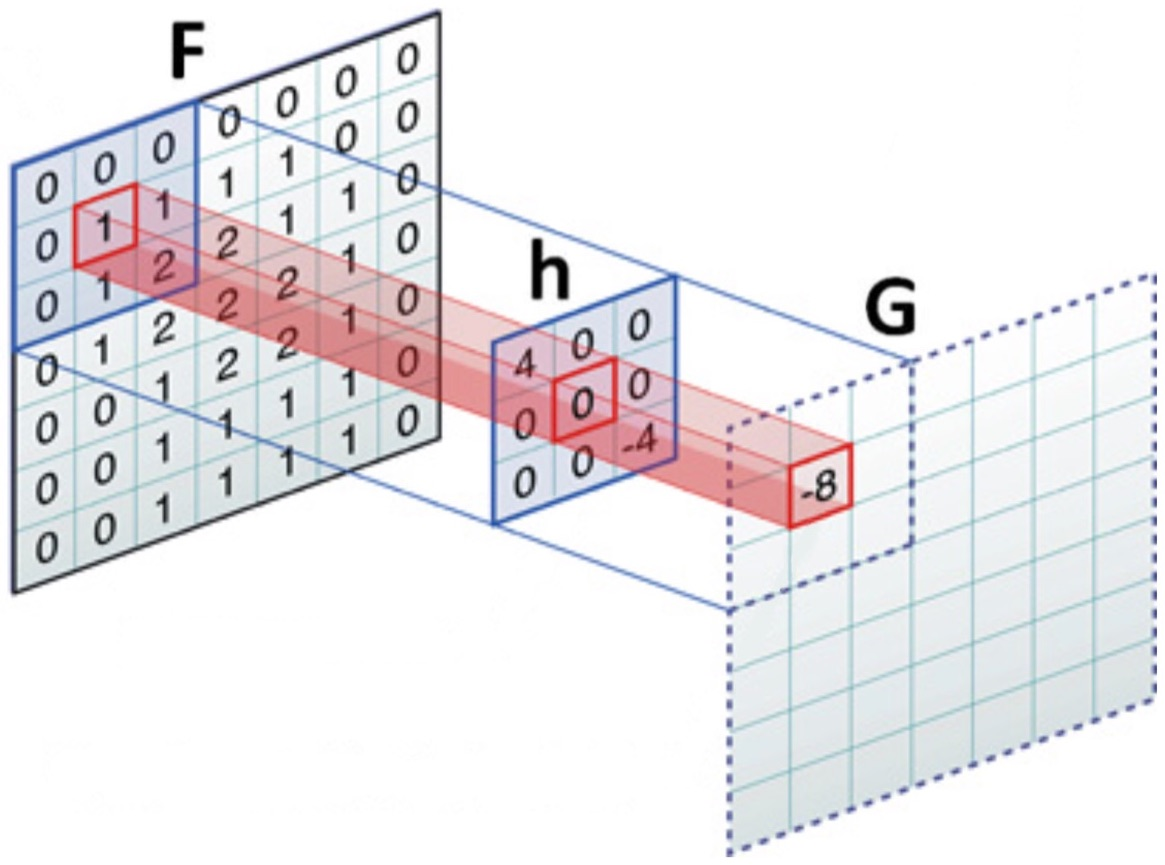
\includegraphics[width=0.6\linewidth]{conv}
   	\end{center}
   	\caption{Свертка матрицы $F$ с ядром свертки $h$.}
   	\label{tikzpicture: conv}
\end{figure}


\indent
\indent
В классическом компьютерном зрении известны конкретные числовые
значения элементов матрицы $h$ для ряда сверток 
специального вида. Например, ядро (чаще называемое оператором) Собеля 
позволяет выделять границы на изображениях, а ядро (чаще
называемое фильтром) Гаусса используется для устранения шума
и размытия контуров на изображении. Идея добавления сверточных слоев в 
 нейронные сети строится на том, что сеть сама в процессе
обучения методом обратного распространения ошибки найдет подходящие
для решения конкретной задачи весовые коэффициенты в обучаемых ядрах.

\indent
\indent
Для полноты изложения отметим, что обычно вместе со сверточными
слоями используются такие 
слои как \textit{Pooling}, \textit{Softmax}, 
\textit{BatchNormalization}\cite{batchnorm}  и \textit{Dropout}\cite{dropout}.


\subsection{Используемые сверточные архитектуры}
\label{section:archs}

\indent
\indent
В данной работе используются следующие архитектуры нейронных сетей:


\begin{itemize}

    \item Residual netwrotk (ResNet) ---
    одна из самых популярных в настоящее время архитектур,
    предложенная в статье от \textit{Microsoft} \cite{resnet}.
    Основная идея состоит в добавлении конкатенации выходов
    слоя с номером  $i$ и слоя с номером $i - 2$ (такая процедура
    получила название \textit{skip connection}). Таким образом авторы
    успешно решают важную проблему 
    обучения глубоких сетей --- затухание градиентов.
    
    \item {Inception} --- топология, предложенная исследователями 
    из компании \textit{Google} \cite{inception}. Основную идею
    можно выразить фразой "сеть внутри сети". Авторы 
    конструируют сеть из блоков \textit{(inception modules)} и
    используют свертки $(1 \times 1)$.
    
    \item {VGG} --- относительно глубокая сеть, авторы которой предложили
    решение проблемы обучения огромного количества параметров
    сверточных слоев \cite{vgg}. Вместо сверток с ядрами $(7 \times 7)$ и
    $(9 \times 9)$ они используют несколько сверток $(3 \times 3)$, таким
    образом уменьшая
    количество весов, но сохраняя 
    площадь восприятия сети \textit{(reception field)}.
    
\end{itemize}

\indent
\indent
Для перечисленных выше архитектур в открытом доступе находятся 
веса обученных моделей, обученных на классификации 1000
категорий датасета \textit{ImageNet}\cite{imagenet}. В настоящей работе
эти веса используются для инициализации весов обучаемых моделей
(для этого требуется заменить размер выходного слоя на количество
хэштегов, рассматриваемых в решаемой задаче).
Такой подход имеет широкое распространение 
и называется \textit{fine-tuning}, он позволяет значительно ускорить
тренировочный процесс и, иногда, увеличить конечную точность модели.

